\documentclass[UTF8,fontset=none,12pt]{ctexart}

\setCJKmainfont{Songti SC}
\setCJKsansfont{PingFang SC}
\setCJKmonofont{Songti SC}

\usepackage[a4paper,margin=2.35cm]{geometry}
\usepackage{amsmath,amssymb,amsthm,mathtools,bm}
\usepackage{graphicx}
\usepackage{float}
\usepackage{booktabs}
\usepackage{array}
\usepackage{enumitem}
\usepackage[hidelinks]{hyperref}

\newcommand{\epsmach}{\varepsilon_{\mathrm{machine}}}

\title{数值线性代数\quad 第 23 讲：Cholesky 分解}
\author{Lloyd N. Trefethen、David Bau III\quad 中文阅读版}
\date{}

\begin{document}
\maketitle
\pagestyle{plain}

Hermitian 正定矩阵可以用三角因子分解，而且运算量只有一般矩阵的
一半。实现这一点的标准算法是 Cholesky 分解。它是高斯消去法的一个
变体，同时在矩阵的左侧和右侧操作，从而保持并利用对称结构。

\section*{Hermitian 正定矩阵}

实矩阵 $A\in\mathbb{R}^{m\times m}$ 如果关于主对角线对称，即
$a_{ij}=a_{ji}$，就称为对称矩阵，因而 $A=A^T$。这样的矩阵满足
\[
x^TAy=y^TAx,\qquad x,y\in\mathbb{R}^m.
\]

对复矩阵 $A\in\mathbb{C}^{m\times m}$，相应的性质是 Hermitian 性：
主对角线下方的条目是主对角线上方对应条目的复共轭，
$a_{ij}=\overline{a_{ji}}$，因而 $A=A^*$。（这些定义已经在第 2 讲
出现过。）注意，Hermitian 矩阵的对角线条目必为实数。

Hermitian 矩阵满足
\[
x^*Ay=y^*Ax,\qquad x,y\in\mathbb{C}^m.
\]
特别地，对任意 $x\in\mathbb{C}^m$，$x^*Ax$ 都是实数。如果进一步
对所有 $x\ne0$ 都有 $x^*Ax>0$，则称 $A$ 为 Hermitian 正定矩阵，
有时也简称正定矩阵。物理系统中出现的许多矩阵，由于基本物理定律，
都是 Hermitian 正定的。

设 $A$ 是 $m\times m$ 的 Hermitian 正定矩阵，$X$ 是满列秩的
$m\times n$ 矩阵，且 $m\ge n$。那么 $X^*AX$ 也是 Hermitian 正定的。
它是 Hermitian 矩阵，因为
\[
(X^*AX)^*=X^*A^*X=X^*AX.
\]
它是正定的，因为对任意 $x\ne0$，有 $Xx\ne0$，从而
\[
x^*(X^*AX)x=(Xx)^*A(Xx)>0.
\]
取每列只有一个 1、其余元素为 0 的 $X$，可以把 $A$ 的任意主子矩阵
写成 $X^*AX$。因此，$A$ 的任意主子矩阵都必须正定；特别地，
$A$ 的每个对角线条目都是正实数。

Hermitian 正定矩阵的特征值也都是正实数。若
$Ax=\lambda x$ 且 $x\ne0$，则
\[
x^*Ax=\lambda x^*x>0,
\]
所以 $\lambda>0$。反过来可以证明，如果 Hermitian 矩阵的全部特征值
为正，那么它就是正定的。

Hermitian 矩阵对应于不同特征值的特征向量彼此正交。
（下一讲会讨论，Hermitian 矩阵是正规矩阵。）设
$Ax_1=\lambda_1x_1$、$Ax_2=\lambda_2x_2$ 且 $\lambda_1\ne\lambda_2$。
那么
\[
\lambda_2x_1^*x_2=x_1^*Ax_2=x_2^*Ax_1
=\overline{\lambda_1}x_2^*x_1=\lambda_1x_1^*x_2,
\]
于是 $(\lambda_1-\lambda_2)x_1^*x_2=0$，从而
$x_1^*x_2=0$。

\section*{对称高斯消去}

现在讨论如何把 Hermitian 正定矩阵分解为三角因子。先考察一个
左上角为 1 的 Hermitian 矩阵，对它执行一步高斯消去：
\[
A=
\begin{bmatrix}
1&w^*\\
w&K
\end{bmatrix}
=
\begin{bmatrix}
1&0\\
w&I
\end{bmatrix}
\begin{bmatrix}
1&w^*\\
0&K-ww^*
\end{bmatrix}.
\]
正如第 20 讲所述，左侧的初等下三角操作从后续各行中减去第一行
的适当倍数，从而在矩阵的第一列引入零。

普通高斯消去法接下来会继续在第二列引入零。不过，为了保持对称性，
Cholesky 分解首先在第一行引入与第一列相匹配的零。可以通过右侧的
上三角操作做到这一点，即从后续各列中减去第一列的适当倍数：
\[
\begin{bmatrix}
1&w^*\\
0&K-ww^*
\end{bmatrix}
=
\begin{bmatrix}
1&0\\
0&K-ww^*
\end{bmatrix}
\begin{bmatrix}
1&w^*\\
0&I
\end{bmatrix}.
\]
注意，这个上三角操作恰好是前面用来在第一列引入零的下三角操作的
伴随。把两个操作合并，得到
\begin{equation}
A=
\begin{bmatrix}
1&0\\
w&I
\end{bmatrix}
\begin{bmatrix}
1&0\\
0&K-ww^*
\end{bmatrix}
\begin{bmatrix}
1&w^*\\
0&I
\end{bmatrix}.
\tag{23.1}
\end{equation}
Cholesky 分解的思想，就是以这种方式继续进行：对 $A$ 的一列和一行
同时引入零，直到它被化为单位矩阵。

\section*{Cholesky 分解}

为了使这种对称三角化对一般情形都有效，我们需要允许任意
$a_{11}>0$，而不只是 $a_{11}=1$。在 (23.1) 中把 $R_1$ 的某些元素
乘以 $\sqrt{a_{11}}$ 即可完成推广。令
$\alpha=\sqrt{a_{11}}$，则
\[
\begin{aligned}
A&=
\begin{bmatrix}
a_{11}&w^*\\
w&K
\end{bmatrix}\\
&=
\begin{bmatrix}
\alpha&0\\
w/\alpha&I
\end{bmatrix}
\begin{bmatrix}
1&0\\
0&K-ww^*/a_{11}
\end{bmatrix}
\begin{bmatrix}
\alpha&w^*/\alpha\\
0&I
\end{bmatrix}
=R_1^*A_1R_1.
\end{aligned}
\]
这就是 Cholesky 分解反复使用的基本步骤。如果子矩阵
$K-ww^*/a_{11}$ 的左上角条目为正，就可以对它使用同一个公式。
于是 $A_1=R_2^*A_2R_2$，从而
$A=R_1^*R_2^*A_2R_2R_1$。继续到右下角，最终得到
\begin{equation}
A=R_1^*R_2^*\cdots R_m^*R_m\cdots R_2R_1.
\tag{23.2}
\end{equation}
把前半段记作 $R^*$、后半段记作 $R$，就有
\begin{equation}
A=R^*R,\qquad r_{jj}>0,
\tag{23.3}
\end{equation}
其中 $R$ 是上三角矩阵。Hermitian 正定矩阵的这种分解称为
Cholesky 分解。

上面的描述还留下一个问题：我们怎么知道子矩阵
$K-ww^*/a_{11}$ 的左上角条目为正？答案是，它必须为正，因为
$K-ww^*/a_{11}$ 是正定的。事实上，它是正定矩阵
$R_1^{-*}AR_1^{-1}$ 的右下角 $(m-1)\times(m-1)$ 主子矩阵。
用归纳法可以得到，在分解过程中出现的所有子矩阵 $A_i$ 都是正定的，
因此算法不可能中途失败。

\paragraph{定理 23.1.}
每个 Hermitian 正定矩阵 $A\in\mathbb{C}^{m\times m}$ 都有唯一的
Cholesky 分解 (23.3)。

\paragraph{证明.}
存在性正是上面的讨论：算法不可能失败，所以分解一定存在。
事实上，算法也给出了唯一性。在每一步 (23.2) 中，
$\alpha=\sqrt{a_{11}}$ 的值由 $R^*R$ 的形式唯一确定；一旦 $\alpha$
确定，$R_1^*$ 的第一行也唯一确定。每一步都如此，因此整个分解唯一。
\hfill$\square$

\section*{算法}

实现 Cholesky 分解时，只需要显式存储正在操作的矩阵的一半，
因而可以省去一半算术运算。下面给出算法的一种正式写法。
输入矩阵 $A$ 表示待分解的 $m\times m$ Hermitian 正定矩阵的上三角部分；
实际软件可以使用压缩存储，避免浪费方阵数组的一半空间。输出矩阵
$R$ 是满足 $A=R^*R$ 的上三角因子。每次外层迭代对应一次基本分解；
在第 $k$ 步，子矩阵 $R_{k:m,k:m}^*$ 的上三角部分表示当前待分解的
Hermitian 矩阵的上三角部分。

\paragraph{算法 23.1（Cholesky 分解）}
\begin{verbatim}
R = A
for k = 1 to m
    for j = k+1 to m
        R(j,j:m) = R(j,j:m) - R(k,j:m)*R(k,j)/R(k,k)
    R(k,k:m) = R(k,k:m)/sqrt(R(k,k))
\end{verbatim}

\section*{运算量}

Cholesky 分解的算术量主要集中在内层循环。内层语句
\[
R_{j,j:m}=R_{j,j:m}-R_{k,j:m}R_{kj}/R_{kk}
\]
每执行一次，需要一次除法、$m-j+1$ 次乘法和 $m-j+1$ 次减法，
总计约 $2(m-j)$ 次浮点运算。对每个 $j=k+1,\ldots,m$ 重复，
再对每个 $k=1,\ldots,m$ 重复。因此
\[
\begin{aligned}
\sum_{k=1}^{m}\sum_{j=k+1}^{m}2(m-j)
&\sim 2\sum_{k=1}^{m}\sum_{j=1}^{k}j
\sim\sum_{k=1}^{m}k^2\\
&\sim\frac13m^3\ \text{flops}.
\end{aligned}
\]
所以，Cholesky 分解的运算量只有高斯消去法的一半；对同一个矩阵，
高斯消去法需要约 $\frac23m^3$ 次浮点运算。

运算量也可以用几何方式计算。对每个 $k$，三角层的每个位置进行两次
浮点运算（一次乘法和一次减法）。整个算法相当于堆叠 $m$ 层：

\begin{figure}[H]
    \centering
    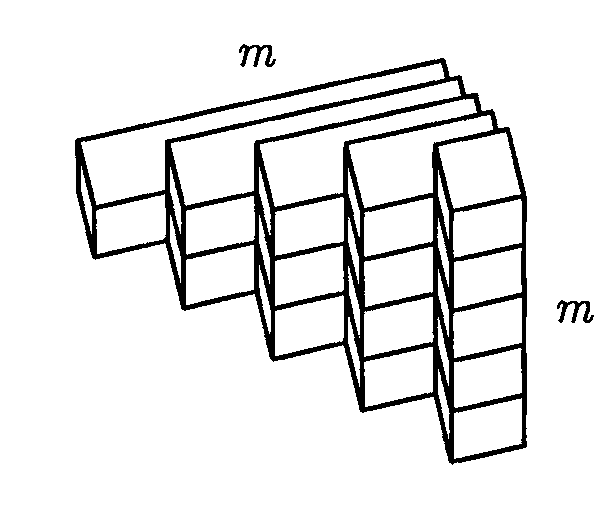
\includegraphics[width=0.58\linewidth]{../assets/figure-23-operation-count.png}
    \caption{Cholesky 分解运算量的几何示意图。}
\end{figure}

当 $m\to\infty$ 时，这个实体趋近于体积为 $\frac16m^3$ 的四面体。
由于每个单位立方体对应两次浮点运算，再次得到
\begin{equation}
\text{Cholesky 分解的工作量}\sim\frac13m^3\ \text{flops}.
\tag{23.4}
\end{equation}

\section*{稳定性}

高斯消去法稳定性分析中的所有微妙之处，在 Cholesky 分解中都消失了。
这个算法总是稳定的。直观地说，这是因为因子 $R$ 不可能变得很大。
例如在 2-范数下，
\[
\|R\|=\|R^*\|=\|A\|^{1/2},
\]
其中等式可由奇异值分解证明；对满足 $1\le p\le\infty$ 的其他
$p$-范数，$\|R\|$ 与 $\|A\|^{1/2}$ 的差别也不会超过一个
$\sqrt m$ 的因子。因此，远大于 $A$ 的条目不可能在计算中出现。

注意，Cholesky 分解不需要任何选主元就能保持稳定。直观上，这与
Hermitian 正定矩阵的大部分权重集中在对角线上有关。例如不难证明，
最大条目必定出现在对角线上；而这个性质也会传递给归纳过程 (23.2)
中构造出的正定子矩阵。

对 Cholesky 过程进行稳定性分析，可以得到下面的向后稳定性结论。

\paragraph{定理 23.2.}
设 $A\in\mathbb{C}^{m\times m}$ 是 Hermitian 正定矩阵，并在满足
(13.5) 和 (13.7) 的计算机上利用算法 23.1 计算其 Cholesky 分解。
当 $\epsmach$ 足够小时，该过程保证完成（不会出现零或负的角元素
$r_{kk}$），并产生满足下式的计算因子 $\widetilde R$：
\begin{equation}
\widetilde R^*\widetilde R=A+\delta A,\qquad
\frac{\|\delta A\|}{\|A\|}=O(\epsmach),
\qquad \delta A\in\mathbb{C}^{m\times m}.
\tag{23.5}
\end{equation}

如果 $A$ 病态，$\widetilde R$ 通常不会接近 $R$；我们最多只能说
\[
\frac{\|\widetilde R-R\|}{\|R\|}
=O\bigl(\kappa(A)\epsmach\bigr).
\]
换句话说，Cholesky 分解一般是一个病态问题。真正满足较好误差界
(23.5) 的是乘积 $\widetilde R^*\widetilde R$。因此，$\widetilde R$
中的舍入误差虽然可能很大，却是“恶魔般相关”的，正如第 16 讲
QR 分解中看到的那样。

\section*{求解 $Ax=b$}

如果 $A$ 是 Hermitian 正定矩阵，求解方程组 $Ax=b$ 的标准方法就是
Cholesky 分解。算法 23.1 把方程组化为
\[
R^*Rx=b,
\]
然后依次求解两个三角方程组：先求未知量 $y$，
$R^*y=b$；再求未知量 $x$，$Rx=y$。每次三角求解只需约
$\frac12m^2$ 次浮点运算，所以总工作量仍为约
$\frac13m^3$ 次浮点运算。

按照与第 16 讲类似的推理，可以证明这个过程是向后稳定的。

\paragraph{定理 23.3.}
通过 Cholesky 分解（算法 23.1）求解 Hermitian 正定方程组
$Ax=b$ 是向后稳定的；所得计算解 $\widetilde x$ 满足
\begin{equation}
(A+\Delta A)\widetilde x=b,\qquad
\frac{\|\Delta A\|}{\|A\|}=O(\epsmach),
\qquad \Delta A\in\mathbb{C}^{m\times m}.
\tag{23.6}
\end{equation}

\section*{习题}

\begin{enumerate}[label=\textbf{23.\arabic*.},leftmargin=*]
    \item 设 $A$ 是非奇异方阵，并设 $A=QR$、$A^*A=U^*U$
    分别是 QR 分解和 Cholesky 分解，且采用通常的归一化
    $r_{jj},u_{jj}>0$。$R=U$ 是真还是假？

    \item 以定理 16.2 的证明为指导，由定理 23.2 和定理 17.1
    推导定理 23.3。

    \item 反向软件工程：MATLAB 的反斜杠。

    下面的 MATLAB 会话记录了在一台 1991 年制造的工作站上，
    对若干计算测量耗时的一系列测试。对每一项，尝试解释：
    (i) 为什么要进行这个实验；(ii) 为什么会得到这样的结果。
    答案应引用正文中的浮点运算量公式。MATLAB 命令
    help chol 和 help slash 可能会帮助你完成这项侦探工作。

\begin{verbatim}
(a) m = 200; Z = randn(m,m);
    A = Z'*Z; b = randn(m,1);
    tic; x = A\b; toc;
         elapsed_time = 1.0368

(b) tic; x = A\b; toc;
         elapsed_time = 1.0303

(c) A2 = A; A2(m,1) = A2(m,1)/2;
    tic; x = A2\b; toc;
         elapsed_time = 2.0361

(d) I = eye(m,m); emin = min(eig(A));
    A3 = A - .9*emin*I;
    tic; x = A3\b; toc;
         elapsed_time = 1.0362

(e) A4 = A - 1.1*emin*I;
    tic; x = A4\b; toc;
         elapsed_time = 2.9624

(f) A5 = triu(A);
    tic; x = A5\b; toc;
         elapsed_time = 0.1261

(g) A6 = A5; A6(m,1) = A5(1,m);
    tic; x = A6\b; toc;
         elapsed_time = 2.0012
\end{verbatim}
\end{enumerate}

\end{document}
